\documentclass{article}%
\usepackage[T1]{fontenc}%
\usepackage[utf8]{inputenc}%
\usepackage{lmodern}%
\usepackage{textcomp}%
\usepackage{lastpage}%
\usepackage[head=40pt,margin=0.5in,bottom=0.6in]{geometry}%
\usepackage{graphicx}%
%
\title{\textbf{Enfermeros del Iahula en Mérida no perciben salarios desde hace siete meses}}%
\author{EL NACIONAL WEB}%
\date{02/12/2018}%
%
\begin{document}%
\normalsize%
\maketitle%
\textbf{URL: }%
http://www.el{-}nacional.com/noticias/sociedad/enfermeros{-}del{-}iahula{-}merida{-}perciben{-}salarios{-}desde{-}hace{-}siete{-}meses\_261902\newline%
%
\textbf{Periodico: }%
EN, %
ID: %
261902, %
Seccion: %
Sociedad\newline%
%
\textbf{Palabras Claves: }%
Salud, Sociedad\newline%
%
\textbf{Derecho: }%
2.3, %
Otros Derechos: %
, %
Sub Derechos: %
2.3.5\newline%
%
\textbf{EP: }%
SI\newline%
\newline%
%
\textbf{\textit{El personal médico no cuenta con insumos para realizar curas o administrar medicamentos vía sanguínea a los pacientes}}%
\newline%
\newline%
%
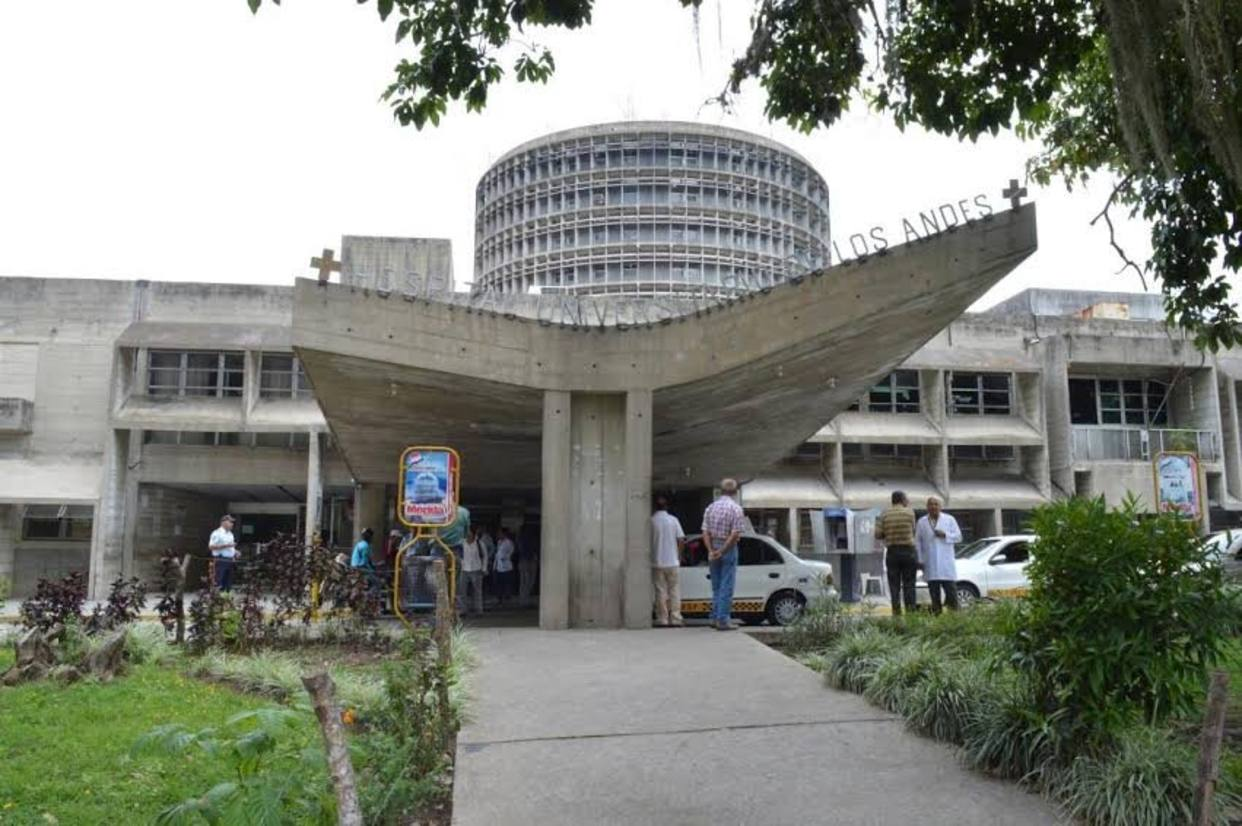
\includegraphics[width=300px]{73.jpg}%
\newline%
%
Enfermeros del Hospital Universitario de Los Andes (Iahula), en Mérida, tienen más de siete meses sin percibir el~salario. Denuncian que no han recibido respuesta de las autoridades competentes ante la falta de pago.%
\newline%
%
Jesús Quintero, periodista, aseguró que el personal no cuenta con los insumos ni implementos necesarios para brindar una atención oportuna a los pacientes que llegan al centro médico. Entre las áreas más afectadas se encuentra la sala de parto y la emergencia obstétrica.%
\newline%
%
Agregó que la entidad no cuenta ni con inyectadoras, algodón o alcohol, por ello~no pueden realizar curas o administrar medicamentos vía sanguínea a los pacientes.%
\newline%
%
\end{document}